\documentclass[twoside]{book}

% Packages required by doxygen
\usepackage{fixltx2e}
\usepackage{calc}
\usepackage{doxygen}
\usepackage[export]{adjustbox} % also loads graphicx
\usepackage{graphicx}
\usepackage[utf8]{inputenc}
\usepackage{makeidx}
\usepackage{multicol}
\usepackage{multirow}
\PassOptionsToPackage{warn}{textcomp}
\usepackage{textcomp}
\usepackage[nointegrals]{wasysym}
\usepackage[table]{xcolor}

% Font selection
\usepackage[T1]{fontenc}
\usepackage[scaled=.90]{helvet}
\usepackage{courier}
\usepackage{amssymb}
\usepackage{sectsty}
\renewcommand{\familydefault}{\sfdefault}
\allsectionsfont{%
  \fontseries{bc}\selectfont%
  \color{darkgray}%
}
\renewcommand{\DoxyLabelFont}{%
  \fontseries{bc}\selectfont%
  \color{darkgray}%
}
\newcommand{\+}{\discretionary{\mbox{\scriptsize$\hookleftarrow$}}{}{}}

% Page & text layout
\usepackage{geometry}
\geometry{%
  a4paper,%
  top=2.5cm,%
  bottom=2.5cm,%
  left=2.5cm,%
  right=2.5cm%
}
\tolerance=750
\hfuzz=15pt
\hbadness=750
\setlength{\emergencystretch}{15pt}
\setlength{\parindent}{0cm}
\setlength{\parskip}{3ex plus 2ex minus 2ex}
\makeatletter
\renewcommand{\paragraph}{%
  \@startsection{paragraph}{4}{0ex}{-1.0ex}{1.0ex}{%
    \normalfont\normalsize\bfseries\SS@parafont%
  }%
}
\renewcommand{\subparagraph}{%
  \@startsection{subparagraph}{5}{0ex}{-1.0ex}{1.0ex}{%
    \normalfont\normalsize\bfseries\SS@subparafont%
  }%
}
\makeatother

% Headers & footers
\usepackage{fancyhdr}
\pagestyle{fancyplain}
\fancyhead[LE]{\fancyplain{}{\bfseries\thepage}}
\fancyhead[CE]{\fancyplain{}{}}
\fancyhead[RE]{\fancyplain{}{\bfseries\leftmark}}
\fancyhead[LO]{\fancyplain{}{\bfseries\rightmark}}
\fancyhead[CO]{\fancyplain{}{}}
\fancyhead[RO]{\fancyplain{}{\bfseries\thepage}}
\fancyfoot[LE]{\fancyplain{}{}}
\fancyfoot[CE]{\fancyplain{}{}}
\fancyfoot[RE]{\fancyplain{}{\bfseries\scriptsize Generated by Doxygen }}
\fancyfoot[LO]{\fancyplain{}{\bfseries\scriptsize Generated by Doxygen }}
\fancyfoot[CO]{\fancyplain{}{}}
\fancyfoot[RO]{\fancyplain{}{}}
\renewcommand{\footrulewidth}{0.4pt}
\renewcommand{\chaptermark}[1]{%
  \markboth{#1}{}%
}
\renewcommand{\sectionmark}[1]{%
  \markright{\thesection\ #1}%
}

% Indices & bibliography
\usepackage{natbib}
\usepackage[titles]{tocloft}
\setcounter{tocdepth}{3}
\setcounter{secnumdepth}{5}
\makeindex

% Hyperlinks (required, but should be loaded last)
\usepackage{ifpdf}
\ifpdf
  \usepackage[pdftex,pagebackref=true]{hyperref}
\else
  \usepackage[ps2pdf,pagebackref=true]{hyperref}
\fi
\hypersetup{%
  colorlinks=true,%
  linkcolor=blue,%
  citecolor=blue,%
  unicode%
}

% Custom commands
\newcommand{\clearemptydoublepage}{%
  \newpage{\pagestyle{empty}\cleardoublepage}%
}

\usepackage{caption}
\captionsetup{labelsep=space,justification=centering,font={bf},singlelinecheck=off,skip=4pt,position=top}

%===== C O N T E N T S =====

\begin{document}

% Titlepage & ToC
\hypersetup{pageanchor=false,
             bookmarksnumbered=true,
             pdfencoding=unicode
            }
\pagenumbering{alph}
\begin{titlepage}
\vspace*{7cm}
\begin{center}%
{\Large My Project }\\
\vspace*{1cm}
{\large Generated by Doxygen 1.8.12}\\
\end{center}
\end{titlepage}
\clearemptydoublepage
\pagenumbering{roman}
\tableofcontents
\clearemptydoublepage
\pagenumbering{arabic}
\hypersetup{pageanchor=true}

%--- Begin generated contents ---
\chapter{Hierarchical Index}
\section{Class Hierarchy}
This inheritance list is sorted roughly, but not completely, alphabetically\+:\begin{DoxyCompactList}
\item \contentsline{section}{A\+N\+FD}{\pageref{struct_a_n_f_d}}{}
\item \contentsline{section}{A\+N\+HE}{\pageref{struct_a_n_h_e}}{}
\item \contentsline{section}{A\+N\+P\+E\+N\+D\+I\+NG}{\pageref{struct_a_n_p_e_n_d_i_n_g}}{}
\item \contentsline{section}{A\+N\+S\+IG}{\pageref{struct_a_n_s_i_g}}{}
\item \contentsline{section}{ev\+\_\+any\+\_\+watcher}{\pageref{unionev__any__watcher}}{}
\item \contentsline{section}{ev\+\_\+async}{\pageref{structev__async}}{}
\item \contentsline{section}{ev\+\_\+check}{\pageref{structev__check}}{}
\item \contentsline{section}{ev\+\_\+child}{\pageref{structev__child}}{}
\item \contentsline{section}{ev\+\_\+cleanup}{\pageref{structev__cleanup}}{}
\item \contentsline{section}{ev\+\_\+embed}{\pageref{structev__embed}}{}
\item \contentsline{section}{ev\+\_\+fork}{\pageref{structev__fork}}{}
\item \contentsline{section}{ev\+\_\+idle}{\pageref{structev__idle}}{}
\item \contentsline{section}{ev\+\_\+io}{\pageref{structev__io}}{}
\item \contentsline{section}{ev\+\_\+loop}{\pageref{structev__loop}}{}
\item \contentsline{section}{ev\+\_\+once}{\pageref{structev__once}}{}
\item \contentsline{section}{ev\+\_\+periodic}{\pageref{structev__periodic}}{}
\item \contentsline{section}{ev\+\_\+prepare}{\pageref{structev__prepare}}{}
\item \contentsline{section}{ev\+\_\+signal}{\pageref{structev__signal}}{}
\item \contentsline{section}{ev\+\_\+stat}{\pageref{structev__stat}}{}
\item \contentsline{section}{ev\+\_\+timer}{\pageref{structev__timer}}{}
\item \contentsline{section}{ev\+\_\+watcher}{\pageref{structev__watcher}}{}
\begin{DoxyCompactList}
\item \contentsline{section}{ev\+:\+:base$<$ ev\+\_\+watcher, watcher $>$}{\pageref{structev_1_1base}}{}
\end{DoxyCompactList}
\item \contentsline{section}{ev\+\_\+watcher\+\_\+list}{\pageref{structev__watcher__list}}{}
\item \contentsline{section}{ev\+\_\+watcher\+\_\+time}{\pageref{structev__watcher__time}}{}
\item \contentsline{section}{ev\+\_\+x\+\_\+once}{\pageref{structev__x__once}}{}
\item \contentsline{section}{event}{\pageref{structevent}}{}
\item \contentsline{section}{event\+\_\+base}{\pageref{structevent__base}}{}
\item \contentsline{section}{ev\+:\+:loop\+\_\+ref}{\pageref{structev_1_1loop__ref}}{}
\begin{DoxyCompactList}
\item \contentsline{section}{ev\+:\+:default\+\_\+loop}{\pageref{structev_1_1default__loop}}{}
\item \contentsline{section}{ev\+:\+:dynamic\+\_\+loop}{\pageref{structev_1_1dynamic__loop}}{}
\end{DoxyCompactList}
\item runtime\+\_\+error\begin{DoxyCompactList}
\item \contentsline{section}{ev\+:\+:bad\+\_\+loop}{\pageref{structev_1_1bad__loop}}{}
\end{DoxyCompactList}
\end{DoxyCompactList}

\chapter{Class Index}
\section{Class List}
Here are the classes, structs, unions and interfaces with brief descriptions\+:\begin{DoxyCompactList}
\item\contentsline{section}{\hyperlink{struct_a_n_f_d}{A\+N\+FD} }{\pageref{struct_a_n_f_d}}{}
\item\contentsline{section}{\hyperlink{struct_a_n_h_e}{A\+N\+HE} }{\pageref{struct_a_n_h_e}}{}
\item\contentsline{section}{\hyperlink{struct_a_n_p_e_n_d_i_n_g}{A\+N\+P\+E\+N\+D\+I\+NG} }{\pageref{struct_a_n_p_e_n_d_i_n_g}}{}
\item\contentsline{section}{\hyperlink{struct_a_n_s_i_g}{A\+N\+S\+IG} }{\pageref{struct_a_n_s_i_g}}{}
\item\contentsline{section}{\hyperlink{structev_1_1bad__loop}{ev\+::bad\+\_\+loop} }{\pageref{structev_1_1bad__loop}}{}
\item\contentsline{section}{\hyperlink{structev_1_1base}{ev\+::base$<$ ev\+\_\+watcher, watcher $>$} }{\pageref{structev_1_1base}}{}
\item\contentsline{section}{\hyperlink{structev_1_1default__loop}{ev\+::default\+\_\+loop} }{\pageref{structev_1_1default__loop}}{}
\item\contentsline{section}{\hyperlink{structev_1_1dynamic__loop}{ev\+::dynamic\+\_\+loop} }{\pageref{structev_1_1dynamic__loop}}{}
\item\contentsline{section}{\hyperlink{unionev__any__watcher}{ev\+\_\+any\+\_\+watcher} }{\pageref{unionev__any__watcher}}{}
\item\contentsline{section}{\hyperlink{structev__async}{ev\+\_\+async} }{\pageref{structev__async}}{}
\item\contentsline{section}{\hyperlink{structev__check}{ev\+\_\+check} }{\pageref{structev__check}}{}
\item\contentsline{section}{\hyperlink{structev__child}{ev\+\_\+child} }{\pageref{structev__child}}{}
\item\contentsline{section}{\hyperlink{structev__cleanup}{ev\+\_\+cleanup} }{\pageref{structev__cleanup}}{}
\item\contentsline{section}{\hyperlink{structev__embed}{ev\+\_\+embed} }{\pageref{structev__embed}}{}
\item\contentsline{section}{\hyperlink{structev__fork}{ev\+\_\+fork} }{\pageref{structev__fork}}{}
\item\contentsline{section}{\hyperlink{structev__idle}{ev\+\_\+idle} }{\pageref{structev__idle}}{}
\item\contentsline{section}{\hyperlink{structev__io}{ev\+\_\+io} }{\pageref{structev__io}}{}
\item\contentsline{section}{\hyperlink{structev__loop}{ev\+\_\+loop} }{\pageref{structev__loop}}{}
\item\contentsline{section}{\hyperlink{structev__once}{ev\+\_\+once} }{\pageref{structev__once}}{}
\item\contentsline{section}{\hyperlink{structev__periodic}{ev\+\_\+periodic} }{\pageref{structev__periodic}}{}
\item\contentsline{section}{\hyperlink{structev__prepare}{ev\+\_\+prepare} }{\pageref{structev__prepare}}{}
\item\contentsline{section}{\hyperlink{structev__signal}{ev\+\_\+signal} }{\pageref{structev__signal}}{}
\item\contentsline{section}{\hyperlink{structev__stat}{ev\+\_\+stat} }{\pageref{structev__stat}}{}
\item\contentsline{section}{\hyperlink{structev__timer}{ev\+\_\+timer} }{\pageref{structev__timer}}{}
\item\contentsline{section}{\hyperlink{structev__watcher}{ev\+\_\+watcher} }{\pageref{structev__watcher}}{}
\item\contentsline{section}{\hyperlink{structev__watcher__list}{ev\+\_\+watcher\+\_\+list} }{\pageref{structev__watcher__list}}{}
\item\contentsline{section}{\hyperlink{structev__watcher__time}{ev\+\_\+watcher\+\_\+time} }{\pageref{structev__watcher__time}}{}
\item\contentsline{section}{\hyperlink{structev__x__once}{ev\+\_\+x\+\_\+once} }{\pageref{structev__x__once}}{}
\item\contentsline{section}{\hyperlink{structevent}{event} }{\pageref{structevent}}{}
\item\contentsline{section}{\hyperlink{structevent__base}{event\+\_\+base} }{\pageref{structevent__base}}{}
\item\contentsline{section}{\hyperlink{structev_1_1loop__ref}{ev\+::loop\+\_\+ref} }{\pageref{structev_1_1loop__ref}}{}
\end{DoxyCompactList}

\chapter{Class Documentation}
\hypertarget{struct_a_n_f_d}{}\section{A\+N\+FD Struct Reference}
\label{struct_a_n_f_d}\index{A\+N\+FD@{A\+N\+FD}}
\subsection*{Public Attributes}
\begin{DoxyCompactItemize}
\item 
\hypertarget{struct_a_n_f_d_a1fd948f270a9e89569e1909f8a5fffaf}{}\label{struct_a_n_f_d_a1fd948f270a9e89569e1909f8a5fffaf} 
\hyperlink{structev__watcher__list}{WL} {\bfseries head}
\item 
\hypertarget{struct_a_n_f_d_aefcc21fd2b58113bd697bf4832a9127d}{}\label{struct_a_n_f_d_aefcc21fd2b58113bd697bf4832a9127d} 
unsigned char {\bfseries events}
\item 
\hypertarget{struct_a_n_f_d_a0f80e417303b92e8826478bfa1225b09}{}\label{struct_a_n_f_d_a0f80e417303b92e8826478bfa1225b09} 
unsigned char {\bfseries reify}
\item 
\hypertarget{struct_a_n_f_d_a8136a4e793913def66f01dd6f6aedc6e}{}\label{struct_a_n_f_d_a8136a4e793913def66f01dd6f6aedc6e} 
unsigned char {\bfseries emask}
\item 
\hypertarget{struct_a_n_f_d_aa5610b4dca18f6fdfcf647cf83b53614}{}\label{struct_a_n_f_d_aa5610b4dca18f6fdfcf647cf83b53614} 
unsigned char {\bfseries unused}
\end{DoxyCompactItemize}


The documentation for this struct was generated from the following file\+:\begin{DoxyCompactItemize}
\item 
ev.\+c\end{DoxyCompactItemize}

\hypertarget{struct_a_n_h_e}{}\section{A\+N\+HE Struct Reference}
\label{struct_a_n_h_e}\index{A\+N\+HE@{A\+N\+HE}}
\subsection*{Public Attributes}
\begin{DoxyCompactItemize}
\item 
\hypertarget{struct_a_n_h_e_ac709e86b847f2ff2c666b76a108be313}{}\label{struct_a_n_h_e_ac709e86b847f2ff2c666b76a108be313} 
ev\+\_\+tstamp {\bfseries at}
\item 
\hypertarget{struct_a_n_h_e_a09752e837045eaebbce3f1a1e2f4274f}{}\label{struct_a_n_h_e_a09752e837045eaebbce3f1a1e2f4274f} 
\hyperlink{structev__watcher__time}{WT} {\bfseries w}
\end{DoxyCompactItemize}


The documentation for this struct was generated from the following file\+:\begin{DoxyCompactItemize}
\item 
ev.\+c\end{DoxyCompactItemize}

\hypertarget{struct_a_n_p_e_n_d_i_n_g}{}\section{A\+N\+P\+E\+N\+D\+I\+NG Struct Reference}
\label{struct_a_n_p_e_n_d_i_n_g}\index{A\+N\+P\+E\+N\+D\+I\+NG@{A\+N\+P\+E\+N\+D\+I\+NG}}
\subsection*{Public Attributes}
\begin{DoxyCompactItemize}
\item 
\hypertarget{struct_a_n_p_e_n_d_i_n_g_a5333be08545d7d50128b62c825cc5923}{}\label{struct_a_n_p_e_n_d_i_n_g_a5333be08545d7d50128b62c825cc5923} 
\hyperlink{structev__watcher}{W} {\bfseries w}
\item 
\hypertarget{struct_a_n_p_e_n_d_i_n_g_ad93f4db748d9b13ac5c8bbb114950761}{}\label{struct_a_n_p_e_n_d_i_n_g_ad93f4db748d9b13ac5c8bbb114950761} 
int {\bfseries events}
\end{DoxyCompactItemize}


The documentation for this struct was generated from the following file\+:\begin{DoxyCompactItemize}
\item 
ev.\+c\end{DoxyCompactItemize}

\hypertarget{struct_a_n_s_i_g}{}\section{A\+N\+S\+IG Struct Reference}
\label{struct_a_n_s_i_g}\index{A\+N\+S\+IG@{A\+N\+S\+IG}}
\subsection*{Public Attributes}
\begin{DoxyCompactItemize}
\item 
\hypertarget{struct_a_n_s_i_g_a989fa99301ecc95e7e8f6084cec5519a}{}\label{struct_a_n_s_i_g_a989fa99301ecc95e7e8f6084cec5519a} 
E\+V\+\_\+\+A\+T\+O\+M\+I\+C\+\_\+T {\bfseries pending}
\item 
\hypertarget{struct_a_n_s_i_g_a705ea8659265dbaff1cd13f43014c655}{}\label{struct_a_n_s_i_g_a705ea8659265dbaff1cd13f43014c655} 
{\bfseries E\+V\+\_\+P}
\item 
\hypertarget{struct_a_n_s_i_g_a4c6de0ed8a0199bbb4c6ef00ccf01546}{}\label{struct_a_n_s_i_g_a4c6de0ed8a0199bbb4c6ef00ccf01546} 
\hyperlink{structev__watcher__list}{WL} {\bfseries head}
\end{DoxyCompactItemize}


The documentation for this struct was generated from the following file\+:\begin{DoxyCompactItemize}
\item 
ev.\+c\end{DoxyCompactItemize}

\hypertarget{structev_1_1bad__loop}{}\section{ev\+:\+:bad\+\_\+loop Struct Reference}
\label{structev_1_1bad__loop}\index{ev\+::bad\+\_\+loop@{ev\+::bad\+\_\+loop}}
Inheritance diagram for ev\+:\+:bad\+\_\+loop\+:\begin{figure}[H]
\begin{center}
\leavevmode
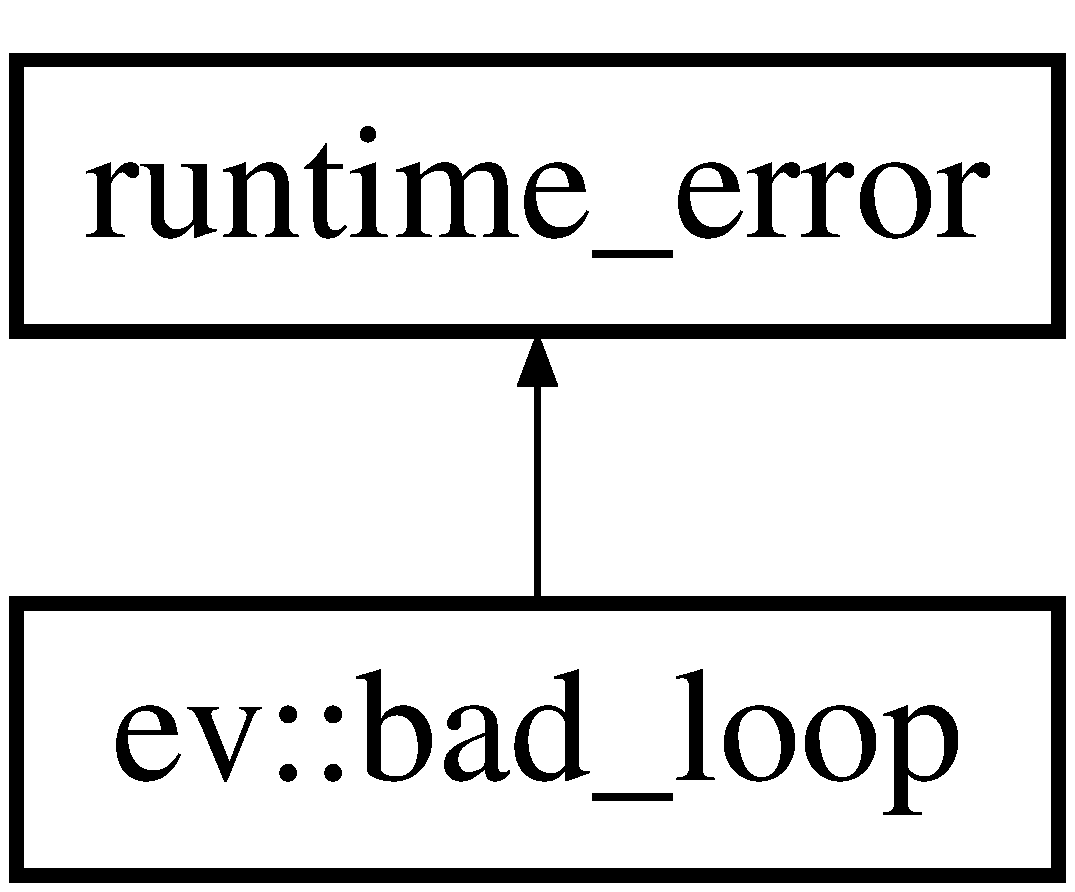
\includegraphics[height=2.000000cm]{structev_1_1bad__loop}
\end{center}
\end{figure}


The documentation for this struct was generated from the following file\+:\begin{DoxyCompactItemize}
\item 
ev++.\+h\end{DoxyCompactItemize}

\hypertarget{structev_1_1base}{}\section{ev\+:\+:base$<$ ev\+\_\+watcher, watcher $>$ Struct Template Reference}
\label{structev_1_1base}\index{ev\+::base$<$ ev\+\_\+watcher, watcher $>$@{ev\+::base$<$ ev\+\_\+watcher, watcher $>$}}
Inheritance diagram for ev\+:\+:base$<$ ev\+\_\+watcher, watcher $>$\+:\begin{figure}[H]
\begin{center}
\leavevmode
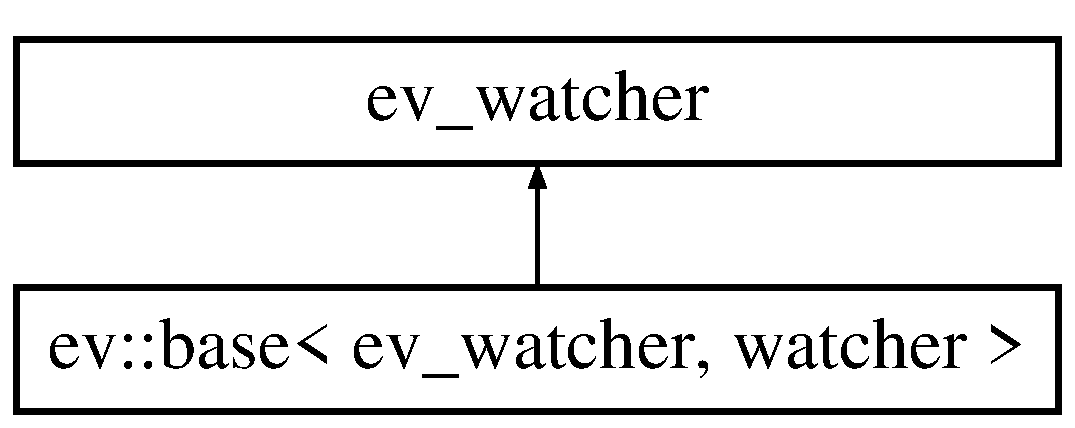
\includegraphics[height=2.000000cm]{structev_1_1base}
\end{center}
\end{figure}
\subsection*{Public Member Functions}
\begin{DoxyCompactItemize}
\item 
\hypertarget{structev_1_1base_acd2c4ed63d3d85fe1503c6a6af79f51f}{}\label{structev_1_1base_acd2c4ed63d3d85fe1503c6a6af79f51f} 
void {\bfseries set} (E\+V\+\_\+P)  throw ()
\item 
\hypertarget{structev_1_1base_ab7bfdea240e4e074f69a330b21839d12}{}\label{structev_1_1base_ab7bfdea240e4e074f69a330b21839d12} 
{\bfseries base} (E\+V\+\_\+\+PX)  throw ()
\item 
\hypertarget{structev_1_1base_af0230caac76aec855cafc1e4a3d8e175}{}\label{structev_1_1base_af0230caac76aec855cafc1e4a3d8e175} 
void {\bfseries set\+\_\+} (const void $\ast$data, void($\ast$cb)(E\+V\+\_\+\+P\+\_\+ \hyperlink{structev__watcher}{ev\+\_\+watcher} $\ast$w, int revents))  throw ()
\item 
\hypertarget{structev_1_1base_aadf4502b7360ca663e9d841d5a8f707a}{}\label{structev_1_1base_aadf4502b7360ca663e9d841d5a8f707a} 
{\footnotesize template$<$void($\ast$)(watcher \&w, int) function$>$ }\\void {\bfseries set} (void $\ast$data=0)  throw ()
\item 
\hypertarget{structev_1_1base_a080c40e6b23fd8027c7a92c218164158}{}\label{structev_1_1base_a080c40e6b23fd8027c7a92c218164158} 
{\footnotesize template$<$class K , void(\+K\+::$\ast$)(watcher \&w, int) method$>$ }\\void {\bfseries set} (K $\ast$object)  throw ()
\item 
\hypertarget{structev_1_1base_a8c76c4def5296155bdc75119628ba6cc}{}\label{structev_1_1base_a8c76c4def5296155bdc75119628ba6cc} 
{\footnotesize template$<$class K $>$ }\\void {\bfseries set} (K $\ast$object)  throw ()
\item 
\hypertarget{structev_1_1base_a080c40e6b23fd8027c7a92c218164158}{}\label{structev_1_1base_a080c40e6b23fd8027c7a92c218164158} 
{\footnotesize template$<$class K , void(\+K\+::$\ast$)() method$>$ }\\void {\bfseries set} (K $\ast$object)  throw ()
\item 
\hypertarget{structev_1_1base_ac4075a29836b2b4f55010e83ce35a38c}{}\label{structev_1_1base_ac4075a29836b2b4f55010e83ce35a38c} 
void {\bfseries operator()} (int events=E\+V\+\_\+\+U\+N\+D\+EF)
\item 
\hypertarget{structev_1_1base_ad05881991b3f36232ec5e62ac11a12c3}{}\label{structev_1_1base_ad05881991b3f36232ec5e62ac11a12c3} 
bool {\bfseries is\+\_\+active} () const  throw ()
\item 
\hypertarget{structev_1_1base_ada2222858acbaa831ddea15eee7c9275}{}\label{structev_1_1base_ada2222858acbaa831ddea15eee7c9275} 
bool {\bfseries is\+\_\+pending} () const  throw ()
\item 
\hypertarget{structev_1_1base_af7e3eb231cd60757cc2c5f97c5ab1015}{}\label{structev_1_1base_af7e3eb231cd60757cc2c5f97c5ab1015} 
void {\bfseries feed\+\_\+event} (int revents)  throw ()
\end{DoxyCompactItemize}
\subsection*{Static Public Member Functions}
\begin{DoxyCompactItemize}
\item 
\hypertarget{structev_1_1base_af92ff4c3ec97e0c58ed6e31ebda29f06}{}\label{structev_1_1base_af92ff4c3ec97e0c58ed6e31ebda29f06} 
{\footnotesize template$<$void($\ast$)(watcher \&w, int) function$>$ }\\static void {\bfseries function\+\_\+thunk} (E\+V\+\_\+\+P\+\_\+ \hyperlink{structev__watcher}{ev\+\_\+watcher} $\ast$w, int revents)
\item 
\hypertarget{structev_1_1base_a92dcb320feed5317236bf538ad5b271d}{}\label{structev_1_1base_a92dcb320feed5317236bf538ad5b271d} 
{\footnotesize template$<$class K , void(\+K\+::$\ast$)(watcher \&w, int) method$>$ }\\static void {\bfseries method\+\_\+thunk} (E\+V\+\_\+\+P\+\_\+ \hyperlink{structev__watcher}{ev\+\_\+watcher} $\ast$w, int revents)
\item 
\hypertarget{structev_1_1base_a50317e6868452f61444c9e2c79ae8aae}{}\label{structev_1_1base_a50317e6868452f61444c9e2c79ae8aae} 
{\footnotesize template$<$class K , void(\+K\+::$\ast$)() method$>$ }\\static void {\bfseries method\+\_\+noargs\+\_\+thunk} (E\+V\+\_\+\+P\+\_\+ \hyperlink{structev__watcher}{ev\+\_\+watcher} $\ast$w, int revents)
\end{DoxyCompactItemize}
\subsection*{Public Attributes}
\begin{DoxyCompactItemize}
\item 
\hypertarget{structev_1_1base_a816642e2a857014212eae34d9696abda}{}\label{structev_1_1base_a816642e2a857014212eae34d9696abda} 
{\bfseries E\+V\+\_\+\+PX}
\end{DoxyCompactItemize}


The documentation for this struct was generated from the following file\+:\begin{DoxyCompactItemize}
\item 
ev++.\+h\end{DoxyCompactItemize}

\hypertarget{structev_1_1default__loop}{}\section{ev\+:\+:default\+\_\+loop Struct Reference}
\label{structev_1_1default__loop}\index{ev\+::default\+\_\+loop@{ev\+::default\+\_\+loop}}
Inheritance diagram for ev\+:\+:default\+\_\+loop\+:\begin{figure}[H]
\begin{center}
\leavevmode
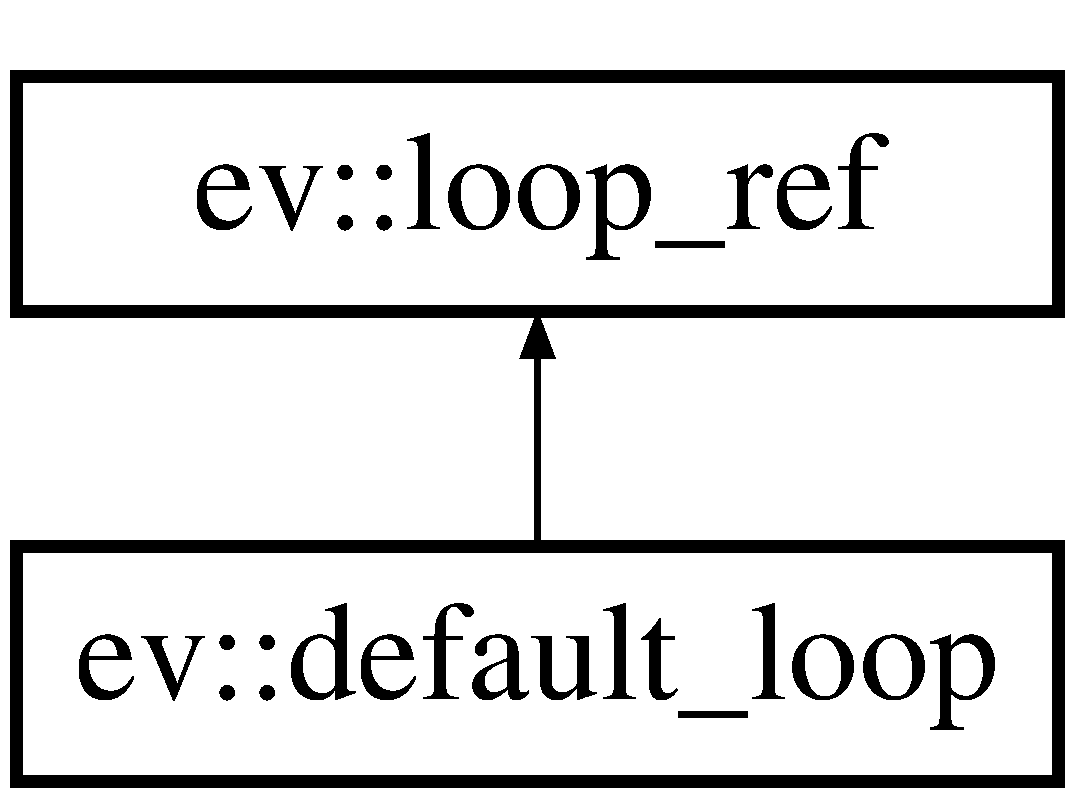
\includegraphics[height=2.000000cm]{structev_1_1default__loop}
\end{center}
\end{figure}
\subsection*{Public Member Functions}
\begin{DoxyCompactItemize}
\item 
\hypertarget{structev_1_1default__loop_a9df32b0a02a3586070fcd093ecd881fa}{}\label{structev_1_1default__loop_a9df32b0a02a3586070fcd093ecd881fa} 
{\bfseries default\+\_\+loop} (unsigned int flags=A\+U\+TO)  throw (bad\+\_\+loop)
\end{DoxyCompactItemize}
\subsection*{Additional Inherited Members}


The documentation for this struct was generated from the following file\+:\begin{DoxyCompactItemize}
\item 
ev++.\+h\end{DoxyCompactItemize}

\hypertarget{structev_1_1dynamic__loop}{}\section{ev\+:\+:dynamic\+\_\+loop Struct Reference}
\label{structev_1_1dynamic__loop}\index{ev\+::dynamic\+\_\+loop@{ev\+::dynamic\+\_\+loop}}
Inheritance diagram for ev\+:\+:dynamic\+\_\+loop\+:\begin{figure}[H]
\begin{center}
\leavevmode
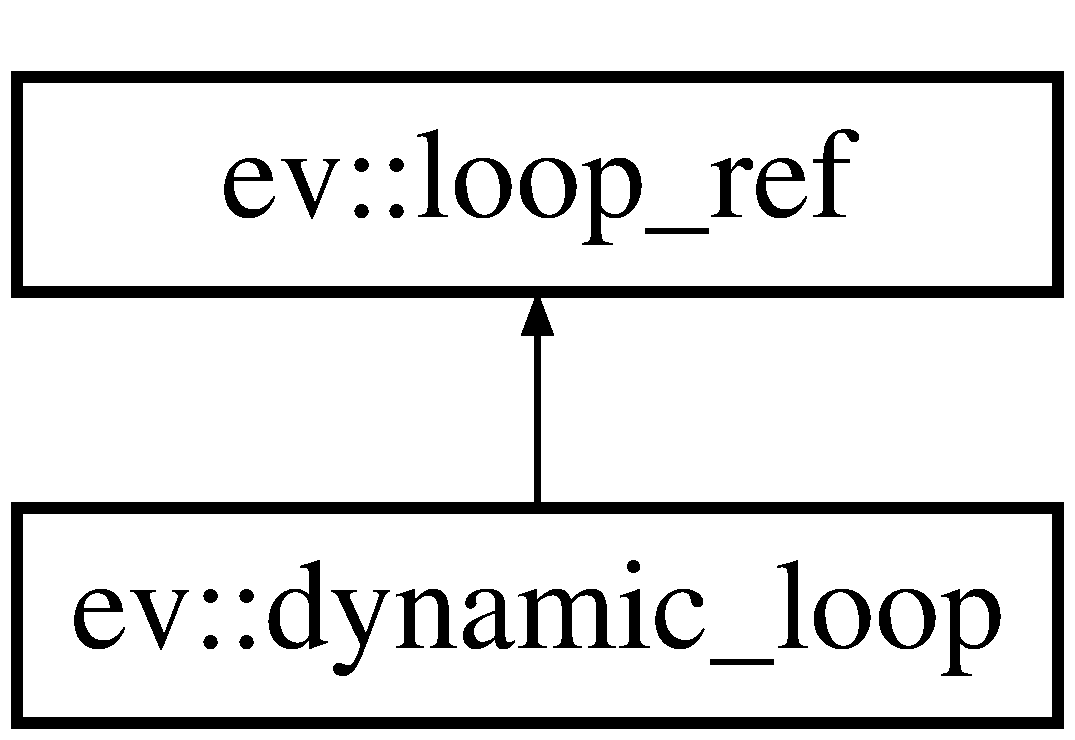
\includegraphics[height=2.000000cm]{structev_1_1dynamic__loop}
\end{center}
\end{figure}
\subsection*{Public Member Functions}
\begin{DoxyCompactItemize}
\item 
\hypertarget{structev_1_1dynamic__loop_ad3d80ce9aef32427a197b4bf8f9a5ca6}{}\label{structev_1_1dynamic__loop_ad3d80ce9aef32427a197b4bf8f9a5ca6} 
{\bfseries dynamic\+\_\+loop} (unsigned int flags=A\+U\+TO)  throw (bad\+\_\+loop)
\end{DoxyCompactItemize}
\subsection*{Additional Inherited Members}


The documentation for this struct was generated from the following file\+:\begin{DoxyCompactItemize}
\item 
ev++.\+h\end{DoxyCompactItemize}

\hypertarget{unionev__any__watcher}{}\section{ev\+\_\+any\+\_\+watcher Union Reference}
\label{unionev__any__watcher}\index{ev\+\_\+any\+\_\+watcher@{ev\+\_\+any\+\_\+watcher}}
\subsection*{Public Attributes}
\begin{DoxyCompactItemize}
\item 
\hypertarget{unionev__any__watcher_a653eb5db584623c06a3c3d55f5d60020}{}\label{unionev__any__watcher_a653eb5db584623c06a3c3d55f5d60020} 
struct \hyperlink{structev__watcher}{ev\+\_\+watcher} {\bfseries w}
\item 
\hypertarget{unionev__any__watcher_a92016edfd8481917f988582d3747f273}{}\label{unionev__any__watcher_a92016edfd8481917f988582d3747f273} 
struct \hyperlink{structev__watcher__list}{ev\+\_\+watcher\+\_\+list} {\bfseries wl}
\item 
\hypertarget{unionev__any__watcher_adf91ee0c0a344e16c3c858a6fe3aacc8}{}\label{unionev__any__watcher_adf91ee0c0a344e16c3c858a6fe3aacc8} 
struct \hyperlink{structev__io}{ev\+\_\+io} {\bfseries io}
\item 
\hypertarget{unionev__any__watcher_ab4660dcfbdcbff80a395deac1b090eac}{}\label{unionev__any__watcher_ab4660dcfbdcbff80a395deac1b090eac} 
struct \hyperlink{structev__timer}{ev\+\_\+timer} {\bfseries timer}
\item 
\hypertarget{unionev__any__watcher_a8b400cd8e29a2a7c997100711e8ee8a3}{}\label{unionev__any__watcher_a8b400cd8e29a2a7c997100711e8ee8a3} 
struct \hyperlink{structev__periodic}{ev\+\_\+periodic} {\bfseries periodic}
\item 
\hypertarget{unionev__any__watcher_a704684338d9105b9a3f1f87e8e48a776}{}\label{unionev__any__watcher_a704684338d9105b9a3f1f87e8e48a776} 
struct \hyperlink{structev__signal}{ev\+\_\+signal} {\bfseries signal}
\item 
\hypertarget{unionev__any__watcher_a60ac726b969a172eaf42e41dcaf54e81}{}\label{unionev__any__watcher_a60ac726b969a172eaf42e41dcaf54e81} 
struct \hyperlink{structev__child}{ev\+\_\+child} {\bfseries child}
\item 
\hypertarget{unionev__any__watcher_a4daa1c06972b03f1e574012ff85f7849}{}\label{unionev__any__watcher_a4daa1c06972b03f1e574012ff85f7849} 
struct \hyperlink{structev__stat}{ev\+\_\+stat} {\bfseries stat}
\item 
\hypertarget{unionev__any__watcher_a981b4fb4bb0c57edde815eb5c653ab21}{}\label{unionev__any__watcher_a981b4fb4bb0c57edde815eb5c653ab21} 
struct \hyperlink{structev__idle}{ev\+\_\+idle} {\bfseries idle}
\item 
\hypertarget{unionev__any__watcher_ab8e9044b76b083a745fe88887035c5b7}{}\label{unionev__any__watcher_ab8e9044b76b083a745fe88887035c5b7} 
struct \hyperlink{structev__prepare}{ev\+\_\+prepare} {\bfseries prepare}
\item 
\hypertarget{unionev__any__watcher_a11934d4f1f244f75b706db27abfea16e}{}\label{unionev__any__watcher_a11934d4f1f244f75b706db27abfea16e} 
struct \hyperlink{structev__check}{ev\+\_\+check} {\bfseries check}
\item 
\hypertarget{unionev__any__watcher_a63e589011bdf5d405a87b0b452d0aa18}{}\label{unionev__any__watcher_a63e589011bdf5d405a87b0b452d0aa18} 
struct \hyperlink{structev__fork}{ev\+\_\+fork} {\bfseries fork}
\item 
\hypertarget{unionev__any__watcher_acf48afbff0708cefa05cfdb2a3f89c52}{}\label{unionev__any__watcher_acf48afbff0708cefa05cfdb2a3f89c52} 
struct \hyperlink{structev__cleanup}{ev\+\_\+cleanup} {\bfseries cleanup}
\item 
\hypertarget{unionev__any__watcher_adecc46ee7ea240767431d1247109ae87}{}\label{unionev__any__watcher_adecc46ee7ea240767431d1247109ae87} 
struct \hyperlink{structev__embed}{ev\+\_\+embed} {\bfseries embed}
\item 
\hypertarget{unionev__any__watcher_ad0452986b798bbf59f852b3e4d164cfe}{}\label{unionev__any__watcher_ad0452986b798bbf59f852b3e4d164cfe} 
struct \hyperlink{structev__async}{ev\+\_\+async} {\bfseries async}
\end{DoxyCompactItemize}


The documentation for this union was generated from the following file\+:\begin{DoxyCompactItemize}
\item 
ev.\+h\end{DoxyCompactItemize}

\hypertarget{structev__async}{}\section{ev\+\_\+async Struct Reference}
\label{structev__async}\index{ev\+\_\+async@{ev\+\_\+async}}
\subsection*{Public Attributes}
\begin{DoxyCompactItemize}
\item 
\hypertarget{structev__async_a73b397e2c5756bff1403e9273e6dbaf3}{}\label{structev__async_a73b397e2c5756bff1403e9273e6dbaf3} 
E\+V\+\_\+\+A\+T\+O\+M\+I\+C\+\_\+T {\bfseries sent}
\end{DoxyCompactItemize}


The documentation for this struct was generated from the following file\+:\begin{DoxyCompactItemize}
\item 
ev.\+h\end{DoxyCompactItemize}

\hypertarget{structev__check}{}\section{ev\+\_\+check Struct Reference}
\label{structev__check}\index{ev\+\_\+check@{ev\+\_\+check}}


The documentation for this struct was generated from the following file\+:\begin{DoxyCompactItemize}
\item 
ev.\+h\end{DoxyCompactItemize}

\hypertarget{structev__child}{}\section{ev\+\_\+child Struct Reference}
\label{structev__child}\index{ev\+\_\+child@{ev\+\_\+child}}
\subsection*{Public Attributes}
\begin{DoxyCompactItemize}
\item 
\hypertarget{structev__child_adc0be0861d839044ff2791879d23b9da}{}\label{structev__child_adc0be0861d839044ff2791879d23b9da} 
int {\bfseries flags}
\item 
\hypertarget{structev__child_aabe34b18e3fd1e6ad14a24e5c0e5ba13}{}\label{structev__child_aabe34b18e3fd1e6ad14a24e5c0e5ba13} 
int {\bfseries pid}
\item 
\hypertarget{structev__child_affe3dced46abf3638cf24b576c07c955}{}\label{structev__child_affe3dced46abf3638cf24b576c07c955} 
int {\bfseries rpid}
\item 
\hypertarget{structev__child_aac9c76006b1e0139dabae9a13775e775}{}\label{structev__child_aac9c76006b1e0139dabae9a13775e775} 
int {\bfseries rstatus}
\end{DoxyCompactItemize}


The documentation for this struct was generated from the following file\+:\begin{DoxyCompactItemize}
\item 
ev.\+h\end{DoxyCompactItemize}

\hypertarget{structev__cleanup}{}\section{ev\+\_\+cleanup Struct Reference}
\label{structev__cleanup}\index{ev\+\_\+cleanup@{ev\+\_\+cleanup}}


The documentation for this struct was generated from the following file\+:\begin{DoxyCompactItemize}
\item 
ev.\+h\end{DoxyCompactItemize}

\hypertarget{structev__embed}{}\section{ev\+\_\+embed Struct Reference}
\label{structev__embed}\index{ev\+\_\+embed@{ev\+\_\+embed}}
\subsection*{Public Attributes}
\begin{DoxyCompactItemize}
\item 
\hypertarget{structev__embed_acb0b3a48271177125760d6b9914e71a7}{}\label{structev__embed_acb0b3a48271177125760d6b9914e71a7} 
struct \hyperlink{structev__loop}{ev\+\_\+loop} $\ast$ {\bfseries other}
\item 
\hypertarget{structev__embed_ab085dde44a1b194137db275caa1cfaa4}{}\label{structev__embed_ab085dde44a1b194137db275caa1cfaa4} 
\hyperlink{structev__io}{ev\+\_\+io} {\bfseries io}
\item 
\hypertarget{structev__embed_a779a812e0c15c15df660c210ee82fb62}{}\label{structev__embed_a779a812e0c15c15df660c210ee82fb62} 
\hyperlink{structev__prepare}{ev\+\_\+prepare} {\bfseries prepare}
\item 
\hypertarget{structev__embed_a96ff5f39de1b7d6c6ac914933063b2f8}{}\label{structev__embed_a96ff5f39de1b7d6c6ac914933063b2f8} 
\hyperlink{structev__check}{ev\+\_\+check} {\bfseries check}
\item 
\hypertarget{structev__embed_a52f8a6147c42ecfe547a44b1f391762d}{}\label{structev__embed_a52f8a6147c42ecfe547a44b1f391762d} 
\hyperlink{structev__timer}{ev\+\_\+timer} {\bfseries timer}
\item 
\hypertarget{structev__embed_aafa62ad98fab654b15c2128ea4b6b167}{}\label{structev__embed_aafa62ad98fab654b15c2128ea4b6b167} 
\hyperlink{structev__periodic}{ev\+\_\+periodic} {\bfseries periodic}
\item 
\hypertarget{structev__embed_a133d7aa3da26a48be70e26eb32aed3d7}{}\label{structev__embed_a133d7aa3da26a48be70e26eb32aed3d7} 
\hyperlink{structev__idle}{ev\+\_\+idle} {\bfseries idle}
\item 
\hypertarget{structev__embed_ad1d0209f5e2006e373028e8cb206c10b}{}\label{structev__embed_ad1d0209f5e2006e373028e8cb206c10b} 
\hyperlink{structev__fork}{ev\+\_\+fork} {\bfseries fork}
\item 
\hypertarget{structev__embed_ac072a5985c406408336aad8b1178ed13}{}\label{structev__embed_ac072a5985c406408336aad8b1178ed13} 
\hyperlink{structev__cleanup}{ev\+\_\+cleanup} {\bfseries cleanup}
\end{DoxyCompactItemize}


The documentation for this struct was generated from the following file\+:\begin{DoxyCompactItemize}
\item 
ev.\+h\end{DoxyCompactItemize}

\hypertarget{structev__fork}{}\section{ev\+\_\+fork Struct Reference}
\label{structev__fork}\index{ev\+\_\+fork@{ev\+\_\+fork}}


The documentation for this struct was generated from the following file\+:\begin{DoxyCompactItemize}
\item 
ev.\+h\end{DoxyCompactItemize}

\hypertarget{structev__idle}{}\section{ev\+\_\+idle Struct Reference}
\label{structev__idle}\index{ev\+\_\+idle@{ev\+\_\+idle}}


The documentation for this struct was generated from the following file\+:\begin{DoxyCompactItemize}
\item 
ev.\+h\end{DoxyCompactItemize}

\hypertarget{structev__io}{}\section{ev\+\_\+io Struct Reference}
\label{structev__io}\index{ev\+\_\+io@{ev\+\_\+io}}
\subsection*{Public Attributes}
\begin{DoxyCompactItemize}
\item 
\hypertarget{structev__io_a5c7e481bb08731a54a00c341d3fccb69}{}\label{structev__io_a5c7e481bb08731a54a00c341d3fccb69} 
int {\bfseries fd}
\item 
\hypertarget{structev__io_a439e3de48a504c0a64cc710338ce1349}{}\label{structev__io_a439e3de48a504c0a64cc710338ce1349} 
int {\bfseries events}
\end{DoxyCompactItemize}


The documentation for this struct was generated from the following file\+:\begin{DoxyCompactItemize}
\item 
ev.\+h\end{DoxyCompactItemize}

\hypertarget{structev__loop}{}\section{ev\+\_\+loop Struct Reference}
\label{structev__loop}\index{ev\+\_\+loop@{ev\+\_\+loop}}
\subsection*{Public Member Functions}
\begin{DoxyCompactItemize}
\item 
\hypertarget{structev__loop_af70c9204d60291f61193b3a35d0933fa}{}\label{structev__loop_af70c9204d60291f61193b3a35d0933fa} 
{\bfseries V\+A\+Rx} (ev\+\_\+tstamp, now\+\_\+floor) V\+A\+Rx(ev\+\_\+tstamp
\item 
\hypertarget{structev__loop_ae65ba4dee55622a0c747d1af4fef6688}{}\label{structev__loop_ae65ba4dee55622a0c747d1af4fef6688} 
mn\+\_\+now {\bfseries V\+A\+Rx} (ev\+\_\+tstamp, rtmn\+\_\+diff) V\+A\+Rx(\hyperlink{structev__watcher}{W} $\ast$
\item 
\hypertarget{structev__loop_a0236d9293613ac338e4d9229929ee4c0}{}\label{structev__loop_a0236d9293613ac338e4d9229929ee4c0} 
mn\+\_\+now rfeeds {\bfseries V\+A\+Rx} (int, rfeedmax) V\+A\+Rx(int
\item 
\hypertarget{structev__loop_ab45749dd490b62f5020de7be6d2fe24b}{}\label{structev__loop_ab45749dd490b62f5020de7be6d2fe24b} 
mn\+\_\+now rfeeds rfeedcnt {\bfseries V\+A\+Rx} (int, pendingpri) V\+A\+Rx(\hyperlink{structev__prepare}{ev\+\_\+prepare}
\item 
\hypertarget{structev__loop_a0be1bf5667b27afedb5e8322811e980a}{}\label{structev__loop_a0be1bf5667b27afedb5e8322811e980a} 
mn\+\_\+now rfeeds rfeedcnt pending\+\_\+w {\bfseries V\+A\+Rx} (ev\+\_\+tstamp, io\+\_\+blocktime) V\+A\+Rx(ev\+\_\+tstamp
\item 
\hypertarget{structev__loop_a81f7380917590214e2632eafeb7e562c}{}\label{structev__loop_a81f7380917590214e2632eafeb7e562c} 
mn\+\_\+now rfeeds rfeedcnt pending\+\_\+w timeout\+\_\+blocktime {\bfseries V\+A\+Rx} (int, backend) V\+A\+Rx(int
\item 
\hypertarget{structev__loop_aa56a1452e06b0cfa8d0846000e18a975}{}\label{structev__loop_aa56a1452e06b0cfa8d0846000e18a975} 
mn\+\_\+now rfeeds rfeedcnt pending\+\_\+w timeout\+\_\+blocktime activecnt {\bfseries V\+A\+Rx} (E\+V\+\_\+\+A\+T\+O\+M\+I\+C\+\_\+T, loop\+\_\+done) V\+A\+Rx(int
\item 
\hypertarget{structev__loop_ac2b18e50e559e782902ab4186dc023c4}{}\label{structev__loop_ac2b18e50e559e782902ab4186dc023c4} 
mn\+\_\+now rfeeds rfeedcnt pending\+\_\+w timeout\+\_\+blocktime activecnt backend\+\_\+fd {\bfseries V\+A\+Rx} (ev\+\_\+tstamp, backend\+\_\+mintime) V\+AR(backend\+\_\+modify
\end{DoxyCompactItemize}
\subsection*{Public Attributes}
\begin{DoxyCompactItemize}
\item 
\hypertarget{structev__loop_a79e0d7a93635df5af6b3d5ee7d0dd613}{}\label{structev__loop_a79e0d7a93635df5af6b3d5ee7d0dd613} 
ev\+\_\+tstamp {\bfseries ev\+\_\+rt\+\_\+now}
\item 
\hypertarget{structev__loop_a638f5a179e4fdca869beb879625038bd}{}\label{structev__loop_a638f5a179e4fdca869beb879625038bd} 
mn\+\_\+now rfeeds rfeedcnt pending\+\_\+w timeout\+\_\+blocktime activecnt backend\+\_\+fd void($\ast$ {\bfseries backend\+\_\+modify} )(E\+V\+\_\+\+P\+\_\+ int fd, int oev, int nev)) V\+AR(backend\+\_\+poll
\item 
\hypertarget{structev__loop_a1214578019211e37965bee8bee4422a5}{}\label{structev__loop_a1214578019211e37965bee8bee4422a5} 
mn\+\_\+now rfeeds rfeedcnt pending\+\_\+w timeout\+\_\+blocktime activecnt backend\+\_\+fd void($\ast$) void($\ast$ {\bfseries backend\+\_\+poll} )(E\+V\+\_\+\+P\+\_\+ ev\+\_\+tstamp timeout)) V\+A\+Rx(\hyperlink{struct_a_n_f_d}{A\+N\+FD} $\ast$
\item 
\hypertarget{structev__loop_a4f38d64993c8d90bac02b5af805cb7f7}{}\label{structev__loop_a4f38d64993c8d90bac02b5af805cb7f7} 
mn\+\_\+now rfeeds rfeedcnt pending\+\_\+w timeout\+\_\+blocktime activecnt backend\+\_\+fd void($\ast$) void($\ast$) anfd {\bfseries V\+A\+Rx} )(int, anfdmax) V\+A\+Rx(\hyperlink{structev__io}{ev\+\_\+io}
\item 
\hypertarget{structev__loop_ace4c219a8e711d707721a502cc2783aa}{}\label{structev__loop_ace4c219a8e711d707721a502cc2783aa} 
mn\+\_\+now rfeeds rfeedcnt pending\+\_\+w timeout\+\_\+blocktime activecnt backend\+\_\+fd void($\ast$) void($\ast$) anfds pipe\+\_\+ {\bfseries V\+A\+Rx} )(E\+V\+\_\+\+A\+T\+O\+M\+I\+C\+\_\+T, pipe\+\_\+write\+\_\+wanted) V\+A\+Rx(E\+V\+\_\+\+A\+T\+O\+M\+I\+C\+\_\+T
\item 
\hypertarget{structev__loop_a3f00c5b63790f7ad669b81af249c2e0c}{}\label{structev__loop_a3f00c5b63790f7ad669b81af249c2e0c} 
mn\+\_\+now rfeeds rfeedcnt pending\+\_\+w timeout\+\_\+blocktime activecnt backend\+\_\+fd void($\ast$) void($\ast$) anfds pipe\+\_\+w pipe\+\_\+write\+\_\+skippe {\bfseries V\+A\+Rx} )(pid\+\_\+t, curpid) V\+A\+Rx(char
\item 
\hypertarget{structev__loop_a849bac09bf792abde809542ef5c8bb68}{}\label{structev__loop_a849bac09bf792abde809542ef5c8bb68} 
mn\+\_\+now rfeeds rfeedcnt pending\+\_\+w timeout\+\_\+blocktime activecnt backend\+\_\+fd void($\ast$) void($\ast$) anfds pipe\+\_\+w pipe\+\_\+write\+\_\+skipped postfor {\bfseries V\+A\+Rx} )(int $\ast$, fdchanges) V\+A\+Rx(int
\item 
\hypertarget{structev__loop_a0fa9e47acaf81489e0dd8bc5b90dd254}{}\label{structev__loop_a0fa9e47acaf81489e0dd8bc5b90dd254} 
mn\+\_\+now rfeeds rfeedcnt pending\+\_\+w timeout\+\_\+blocktime activecnt backend\+\_\+fd void($\ast$) void($\ast$) anfds pipe\+\_\+w pipe\+\_\+write\+\_\+skipped postfork fdchangema {\bfseries V\+A\+Rx} )(int, fdchangecnt) V\+A\+Rx(\hyperlink{struct_a_n_h_e}{A\+N\+HE} $\ast$
\item 
\hypertarget{structev__loop_a6f56555476bcf149cbdcffb172f48319}{}\label{structev__loop_a6f56555476bcf149cbdcffb172f48319} 
mn\+\_\+now rfeeds rfeedcnt pending\+\_\+w timeout\+\_\+blocktime activecnt backend\+\_\+fd void($\ast$) void($\ast$) anfds pipe\+\_\+w pipe\+\_\+write\+\_\+skipped postfork fdchangemax timer {\bfseries V\+A\+Rx} )(int, timermax) V\+A\+Rx(int
\item 
\hypertarget{structev__loop_a4743a441179a66c19db719bcb9726abd}{}\label{structev__loop_a4743a441179a66c19db719bcb9726abd} 
mn\+\_\+now rfeeds rfeedcnt pending\+\_\+w timeout\+\_\+blocktime activecnt backend\+\_\+fd void($\ast$) void($\ast$) anfds pipe\+\_\+w pipe\+\_\+write\+\_\+skipped postfork fdchangemax timers timercn {\bfseries V\+A\+Rx} )(\hyperlink{struct_a_n_h_e}{A\+N\+HE} $\ast$, periodics) V\+A\+Rx(int
\item 
\hypertarget{structev__loop_ae7f845d72a332dc09fc58bc9bff84c5f}{}\label{structev__loop_ae7f845d72a332dc09fc58bc9bff84c5f} 
mn\+\_\+now rfeeds rfeedcnt pending\+\_\+w timeout\+\_\+blocktime activecnt backend\+\_\+fd void($\ast$) void($\ast$) anfds pipe\+\_\+w pipe\+\_\+write\+\_\+skipped postfork fdchangemax timers timercnt periodicma {\bfseries V\+A\+Rx} )(int, periodiccnt) V\+A\+Rx(int
\item 
\hypertarget{structev__loop_a5943a455162c6f045b8653971c6b2ada}{}\label{structev__loop_a5943a455162c6f045b8653971c6b2ada} 
mn\+\_\+now rfeeds rfeedcnt pending\+\_\+w timeout\+\_\+blocktime activecnt backend\+\_\+fd void($\ast$) void($\ast$) anfds pipe\+\_\+w pipe\+\_\+write\+\_\+skipped postfork fdchangemax timers timercnt periodicmax idleal {\bfseries V\+A\+Rx} )(struct \hyperlink{structev__prepare}{ev\+\_\+prepare} $\ast$$\ast$, prepares) V\+A\+Rx(int
\item 
\hypertarget{structev__loop_adf89c4ecb8abadec6860df9077bc1b93}{}\label{structev__loop_adf89c4ecb8abadec6860df9077bc1b93} 
mn\+\_\+now rfeeds rfeedcnt pending\+\_\+w timeout\+\_\+blocktime activecnt backend\+\_\+fd void($\ast$) void($\ast$) anfds pipe\+\_\+w pipe\+\_\+write\+\_\+skipped postfork fdchangemax timers timercnt periodicmax idleall preparema {\bfseries V\+A\+Rx} )(int, preparecnt) V\+A\+Rx(struct \hyperlink{structev__check}{ev\+\_\+check} $\ast$$\ast$
\item 
\hypertarget{structev__loop_a4385a0d394340966d4536baffcf78a94}{}\label{structev__loop_a4385a0d394340966d4536baffcf78a94} 
mn\+\_\+now rfeeds rfeedcnt pending\+\_\+w timeout\+\_\+blocktime activecnt backend\+\_\+fd void($\ast$) void($\ast$) anfds pipe\+\_\+w pipe\+\_\+write\+\_\+skipped postfork fdchangemax timers timercnt periodicmax idleall preparemax check {\bfseries V\+A\+Rx} )(int, checkmax) V\+A\+Rx(int
\item 
\hypertarget{structev__loop_a6b457b9b4e0643f6b322cf5f44815e27}{}\label{structev__loop_a6b457b9b4e0643f6b322cf5f44815e27} 
mn\+\_\+now rfeeds rfeedcnt pending\+\_\+w timeout\+\_\+blocktime activecnt backend\+\_\+fd void($\ast$) void($\ast$) anfds pipe\+\_\+w pipe\+\_\+write\+\_\+skipped postfork fdchangemax timers timercnt periodicmax idleall preparemax checks checkcn {\bfseries V\+A\+Rx} )(struct \hyperlink{structev__fork}{ev\+\_\+fork} $\ast$$\ast$, forks) V\+A\+Rx(int
\item 
\hypertarget{structev__loop_a2b95ab2c8bc3f04480910fd8c6b64038}{}\label{structev__loop_a2b95ab2c8bc3f04480910fd8c6b64038} 
mn\+\_\+now rfeeds rfeedcnt pending\+\_\+w timeout\+\_\+blocktime activecnt backend\+\_\+fd void($\ast$) void($\ast$) anfds pipe\+\_\+w pipe\+\_\+write\+\_\+skipped postfork fdchangemax timers timercnt periodicmax idleall preparemax checks checkcnt forkma {\bfseries V\+A\+Rx} )(int, forkcnt) V\+A\+Rx(struct \hyperlink{structev__cleanup}{ev\+\_\+cleanup} $\ast$$\ast$
\item 
\hypertarget{structev__loop_a72a84b14c2418a71a23c07d32dcbaa02}{}\label{structev__loop_a72a84b14c2418a71a23c07d32dcbaa02} 
mn\+\_\+now rfeeds rfeedcnt pending\+\_\+w timeout\+\_\+blocktime activecnt backend\+\_\+fd void($\ast$) void($\ast$) anfds pipe\+\_\+w pipe\+\_\+write\+\_\+skipped postfork fdchangemax timers timercnt periodicmax idleall preparemax checks checkcnt forkmax cleanup {\bfseries V\+A\+Rx} )(int, cleanupmax) V\+A\+Rx(int
\item 
\hypertarget{structev__loop_ace8faa58e25a8b0baeea8d166c1ccce1}{}\label{structev__loop_ace8faa58e25a8b0baeea8d166c1ccce1} 
mn\+\_\+now rfeeds rfeedcnt pending\+\_\+w timeout\+\_\+blocktime activecnt backend\+\_\+fd void($\ast$) void($\ast$) anfds pipe\+\_\+w pipe\+\_\+write\+\_\+skipped postfork fdchangemax timers timercnt periodicmax idleall preparemax checks checkcnt forkmax cleanups cleanupcn {\bfseries V\+A\+Rx} )(E\+V\+\_\+\+A\+T\+O\+M\+I\+C\+\_\+T, async\+\_\+pending) V\+A\+Rx(struct \hyperlink{structev__async}{ev\+\_\+async} $\ast$$\ast$
\item 
\hypertarget{structev__loop_a7eedbc2d379e8466b07171230fd401ba}{}\label{structev__loop_a7eedbc2d379e8466b07171230fd401ba} 
mn\+\_\+now rfeeds rfeedcnt pending\+\_\+w timeout\+\_\+blocktime activecnt backend\+\_\+fd void($\ast$) void($\ast$) anfds pipe\+\_\+w pipe\+\_\+write\+\_\+skipped postfork fdchangemax timers timercnt periodicmax idleall preparemax checks checkcnt forkmax cleanups cleanupcnt async {\bfseries V\+A\+Rx} )(int, asyncmax) V\+A\+Rx(int
\item 
\hypertarget{structev__loop_a438c33f65e110684ca3939d0d8e4f8a2}{}\label{structev__loop_a438c33f65e110684ca3939d0d8e4f8a2} 
mn\+\_\+now rfeeds rfeedcnt pending\+\_\+w timeout\+\_\+blocktime activecnt backend\+\_\+fd void($\ast$) void($\ast$) anfds pipe\+\_\+w pipe\+\_\+write\+\_\+skipped postfork fdchangemax timers timercnt periodicmax idleall preparemax checks checkcnt forkmax cleanups cleanupcnt asyncs asynccn {\bfseries V\+A\+Rx} )(E\+V\+\_\+\+A\+T\+O\+M\+I\+C\+\_\+T, sig\+\_\+pending) V\+A\+Rx(unsigned int
\item 
\hypertarget{structev__loop_a11bb08304f0f56cdec463e295b0c9681}{}\label{structev__loop_a11bb08304f0f56cdec463e295b0c9681} 
mn\+\_\+now rfeeds rfeedcnt pending\+\_\+w timeout\+\_\+blocktime activecnt backend\+\_\+fd void($\ast$) void($\ast$) anfds pipe\+\_\+w pipe\+\_\+write\+\_\+skipped postfork fdchangemax timers timercnt periodicmax idleall preparemax checks checkcnt forkmax cleanups cleanupcnt asyncs asynccnt origflag {\bfseries V\+A\+Rx} )(unsigned int, loop\+\_\+count) V\+A\+Rx(unsigned int
\item 
\hypertarget{structev__loop_ad26ec14f78b12783aa70ae5102bce964}{}\label{structev__loop_ad26ec14f78b12783aa70ae5102bce964} 
mn\+\_\+now rfeeds rfeedcnt pending\+\_\+w timeout\+\_\+blocktime activecnt backend\+\_\+fd void($\ast$) void($\ast$) anfds pipe\+\_\+w pipe\+\_\+write\+\_\+skipped postfork fdchangemax timers timercnt periodicmax idleall preparemax checks checkcnt forkmax cleanups cleanupcnt asyncs asynccnt origflags loop\+\_\+dept {\bfseries V\+A\+Rx} )(void $\ast$, userdata) V\+AR(release\+\_\+cb
\item 
\hypertarget{structev__loop_aee33fe4c236c060160b1c589551c14d9}{}\label{structev__loop_aee33fe4c236c060160b1c589551c14d9} 
mn\+\_\+now rfeeds rfeedcnt pending\+\_\+w timeout\+\_\+blocktime activecnt backend\+\_\+fd void($\ast$) void($\ast$) anfds pipe\+\_\+w pipe\+\_\+write\+\_\+skipped postfork fdchangemax timers timercnt periodicmax idleall preparemax checks checkcnt forkmax cleanups cleanupcnt asyncs asynccnt origflags loop\+\_\+depth void($\ast$ {\bfseries release\+\_\+cb} )(E\+V\+\_\+P) E\+V\+\_\+\+T\+H\+R\+OW) V\+AR(acquire\+\_\+cb
\end{DoxyCompactItemize}


The documentation for this struct was generated from the following file\+:\begin{DoxyCompactItemize}
\item 
ev.\+c\end{DoxyCompactItemize}

\hypertarget{structev__once}{}\section{ev\+\_\+once Struct Reference}
\label{structev__once}\index{ev\+\_\+once@{ev\+\_\+once}}
\subsection*{Public Attributes}
\begin{DoxyCompactItemize}
\item 
\hypertarget{structev__once_a79ee568256ee0ea8bafb50c5171dcfa8}{}\label{structev__once_a79ee568256ee0ea8bafb50c5171dcfa8} 
\hyperlink{structev__io}{ev\+\_\+io} {\bfseries io}
\item 
\hypertarget{structev__once_a2bde1f0ab49b7160debb6f8f6c867bdc}{}\label{structev__once_a2bde1f0ab49b7160debb6f8f6c867bdc} 
\hyperlink{structev__timer}{ev\+\_\+timer} {\bfseries to}
\item 
\hypertarget{structev__once_a83917293ed96a4e3d5f8b0aeea496d18}{}\label{structev__once_a83917293ed96a4e3d5f8b0aeea496d18} 
void($\ast$ {\bfseries cb} )(int revents, void $\ast$arg)
\item 
\hypertarget{structev__once_afbd70f51924d91e9bcde63706014010e}{}\label{structev__once_afbd70f51924d91e9bcde63706014010e} 
void $\ast$ {\bfseries arg}
\end{DoxyCompactItemize}


The documentation for this struct was generated from the following file\+:\begin{DoxyCompactItemize}
\item 
ev.\+c\end{DoxyCompactItemize}

\hypertarget{structev__periodic}{}\section{ev\+\_\+periodic Struct Reference}
\label{structev__periodic}\index{ev\+\_\+periodic@{ev\+\_\+periodic}}
\subsection*{Public Attributes}
\begin{DoxyCompactItemize}
\item 
\hypertarget{structev__periodic_ae7fca8b8ce6fbccc41372d7bf12813e6}{}\label{structev__periodic_ae7fca8b8ce6fbccc41372d7bf12813e6} 
ev\+\_\+tstamp {\bfseries offset}
\item 
\hypertarget{structev__periodic_a84e353461763d37229b4a7028ed852aa}{}\label{structev__periodic_a84e353461763d37229b4a7028ed852aa} 
ev\+\_\+tstamp {\bfseries interval}
\item 
\hypertarget{structev__periodic_a2485c7ae4650ce0376fd3b24e71e37f7}{}\label{structev__periodic_a2485c7ae4650ce0376fd3b24e71e37f7} 
ev\+\_\+tstamp($\ast$ {\bfseries reschedule\+\_\+cb} )(struct \hyperlink{structev__periodic}{ev\+\_\+periodic} $\ast$w, ev\+\_\+tstamp now) E\+V\+\_\+\+T\+H\+R\+OW
\end{DoxyCompactItemize}


The documentation for this struct was generated from the following file\+:\begin{DoxyCompactItemize}
\item 
ev.\+h\end{DoxyCompactItemize}

\hypertarget{structev__prepare}{}\section{ev\+\_\+prepare Struct Reference}
\label{structev__prepare}\index{ev\+\_\+prepare@{ev\+\_\+prepare}}


The documentation for this struct was generated from the following file\+:\begin{DoxyCompactItemize}
\item 
ev.\+h\end{DoxyCompactItemize}

\hypertarget{structev__signal}{}\section{ev\+\_\+signal Struct Reference}
\label{structev__signal}\index{ev\+\_\+signal@{ev\+\_\+signal}}
\subsection*{Public Attributes}
\begin{DoxyCompactItemize}
\item 
\hypertarget{structev__signal_a6e2aa67420522727edd77c291bc29cbe}{}\label{structev__signal_a6e2aa67420522727edd77c291bc29cbe} 
int {\bfseries signum}
\end{DoxyCompactItemize}


The documentation for this struct was generated from the following file\+:\begin{DoxyCompactItemize}
\item 
ev.\+h\end{DoxyCompactItemize}

\hypertarget{structev__stat}{}\section{ev\+\_\+stat Struct Reference}
\label{structev__stat}\index{ev\+\_\+stat@{ev\+\_\+stat}}
\subsection*{Public Attributes}
\begin{DoxyCompactItemize}
\item 
\hypertarget{structev__stat_acec38fb069a9dd9c8f57ea1ca0c70076}{}\label{structev__stat_acec38fb069a9dd9c8f57ea1ca0c70076} 
\hyperlink{structev__timer}{ev\+\_\+timer} {\bfseries timer}
\item 
\hypertarget{structev__stat_a41db8a24ee882bd042baef97ca153def}{}\label{structev__stat_a41db8a24ee882bd042baef97ca153def} 
ev\+\_\+tstamp {\bfseries interval}
\item 
\hypertarget{structev__stat_a90d741ec1bba36e053b47d187b8d377e}{}\label{structev__stat_a90d741ec1bba36e053b47d187b8d377e} 
const char $\ast$ {\bfseries path}
\item 
\hypertarget{structev__stat_a1c5c01c31a95d2062385993ce0a931bf}{}\label{structev__stat_a1c5c01c31a95d2062385993ce0a931bf} 
ev\+\_\+statdata {\bfseries prev}
\item 
\hypertarget{structev__stat_a7988df9156ed36966c979ed78e576350}{}\label{structev__stat_a7988df9156ed36966c979ed78e576350} 
ev\+\_\+statdata {\bfseries attr}
\item 
\hypertarget{structev__stat_ad0c919954f8bc21de322381f0821a06f}{}\label{structev__stat_ad0c919954f8bc21de322381f0821a06f} 
int {\bfseries wd}
\end{DoxyCompactItemize}


The documentation for this struct was generated from the following file\+:\begin{DoxyCompactItemize}
\item 
ev.\+h\end{DoxyCompactItemize}

\hypertarget{structev__timer}{}\section{ev\+\_\+timer Struct Reference}
\label{structev__timer}\index{ev\+\_\+timer@{ev\+\_\+timer}}
\subsection*{Public Attributes}
\begin{DoxyCompactItemize}
\item 
\hypertarget{structev__timer_a4d2b34c259adabc6ddc738b89341c249}{}\label{structev__timer_a4d2b34c259adabc6ddc738b89341c249} 
ev\+\_\+tstamp {\bfseries repeat}
\end{DoxyCompactItemize}


The documentation for this struct was generated from the following file\+:\begin{DoxyCompactItemize}
\item 
ev.\+h\end{DoxyCompactItemize}

\hypertarget{structev__watcher}{}\section{ev\+\_\+watcher Struct Reference}
\label{structev__watcher}\index{ev\+\_\+watcher@{ev\+\_\+watcher}}
Inheritance diagram for ev\+\_\+watcher\+:\begin{figure}[H]
\begin{center}
\leavevmode
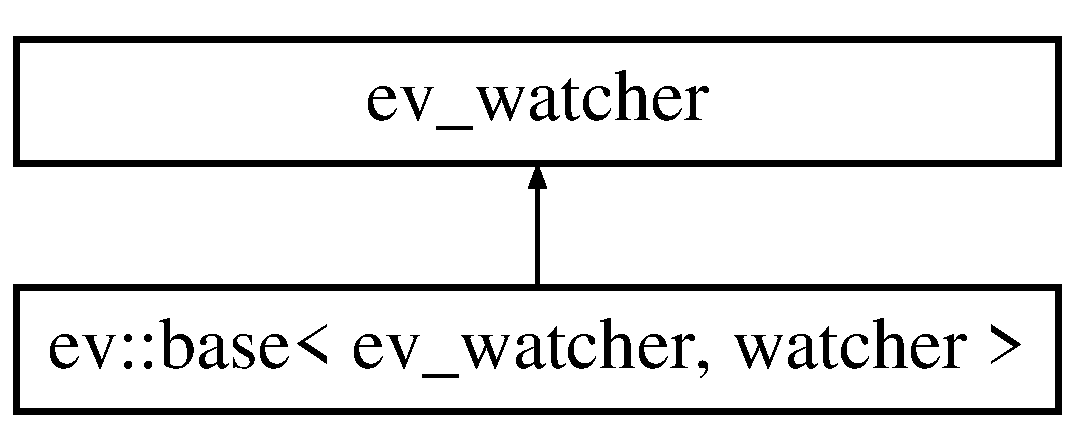
\includegraphics[height=2.000000cm]{structev__watcher}
\end{center}
\end{figure}


The documentation for this struct was generated from the following file\+:\begin{DoxyCompactItemize}
\item 
ev.\+h\end{DoxyCompactItemize}

\hypertarget{structev__watcher__list}{}\section{ev\+\_\+watcher\+\_\+list Struct Reference}
\label{structev__watcher__list}\index{ev\+\_\+watcher\+\_\+list@{ev\+\_\+watcher\+\_\+list}}


The documentation for this struct was generated from the following file\+:\begin{DoxyCompactItemize}
\item 
ev.\+h\end{DoxyCompactItemize}

\hypertarget{structev__watcher__time}{}\section{ev\+\_\+watcher\+\_\+time Struct Reference}
\label{structev__watcher__time}\index{ev\+\_\+watcher\+\_\+time@{ev\+\_\+watcher\+\_\+time}}


The documentation for this struct was generated from the following file\+:\begin{DoxyCompactItemize}
\item 
ev.\+h\end{DoxyCompactItemize}

\hypertarget{structev__x__once}{}\section{ev\+\_\+x\+\_\+once Struct Reference}
\label{structev__x__once}\index{ev\+\_\+x\+\_\+once@{ev\+\_\+x\+\_\+once}}
\subsection*{Public Attributes}
\begin{DoxyCompactItemize}
\item 
\hypertarget{structev__x__once_ad8bab46828192f0962c4c5b523cff7ef}{}\label{structev__x__once_ad8bab46828192f0962c4c5b523cff7ef} 
int {\bfseries fd}
\item 
\hypertarget{structev__x__once_ab55a59ff9bdf70da8f0c6d717ae27b72}{}\label{structev__x__once_ab55a59ff9bdf70da8f0c6d717ae27b72} 
void($\ast$ {\bfseries cb} )(int, short, void $\ast$)
\item 
\hypertarget{structev__x__once_a982a915afeeacdbcf2612bd6da70a2eb}{}\label{structev__x__once_a982a915afeeacdbcf2612bd6da70a2eb} 
void $\ast$ {\bfseries arg}
\end{DoxyCompactItemize}


The documentation for this struct was generated from the following file\+:\begin{DoxyCompactItemize}
\item 
event.\+c\end{DoxyCompactItemize}

\hypertarget{structevent}{}\section{event Struct Reference}
\label{structevent}\index{event@{event}}
\subsection*{Public Attributes}
\begin{DoxyCompactItemize}
\item 
\hypertarget{structevent_a668c11f52e6c54f9e2b7d1aef5bbb363}{}\label{structevent_a668c11f52e6c54f9e2b7d1aef5bbb363} 
\begin{tabbing}
xx\=xx\=xx\=xx\=xx\=xx\=xx\=xx\=xx\=\kill
union \{\\
\>struct \hyperlink{structev__io}{ev\_io} {\bfseries io}\\
\>struct \hyperlink{structev__signal}{ev\_signal} {\bfseries sig}\\
\} {\bfseries iosig}\\

\end{tabbing}\item 
\hypertarget{structevent_a2bc71ca847b882aa99871e53e98769bd}{}\label{structevent_a2bc71ca847b882aa99871e53e98769bd} 
struct \hyperlink{structev__timer}{ev\+\_\+timer} {\bfseries to}
\item 
\hypertarget{structevent_ad0ca55c90047d869af935d02b6bf98d3}{}\label{structevent_ad0ca55c90047d869af935d02b6bf98d3} 
struct \hyperlink{structevent__base}{event\+\_\+base} $\ast$ {\bfseries ev\+\_\+base}
\item 
\hypertarget{structevent_a46ff4af8c64f00fdac8aa8c5e6368438}{}\label{structevent_a46ff4af8c64f00fdac8aa8c5e6368438} 
event\+\_\+callback\+\_\+fn {\bfseries ev\+\_\+callback}
\item 
\hypertarget{structevent_a73daed0b06adc2661c2bb5cac36b6d72}{}\label{structevent_a73daed0b06adc2661c2bb5cac36b6d72} 
void $\ast$ {\bfseries ev\+\_\+arg}
\item 
\hypertarget{structevent_ac4e9ba9d79228d625bd80d441df1b6ef}{}\label{structevent_ac4e9ba9d79228d625bd80d441df1b6ef} 
int {\bfseries ev\+\_\+fd}
\item 
\hypertarget{structevent_a19f9705ccad3d699a67399ca64fcfe4e}{}\label{structevent_a19f9705ccad3d699a67399ca64fcfe4e} 
int {\bfseries ev\+\_\+pri}
\item 
\hypertarget{structevent_a5004429f1cad8ddf9406b48bf1ba6365}{}\label{structevent_a5004429f1cad8ddf9406b48bf1ba6365} 
int {\bfseries ev\+\_\+res}
\item 
\hypertarget{structevent_adb6d076d774729e652c274190036698e}{}\label{structevent_adb6d076d774729e652c274190036698e} 
int {\bfseries ev\+\_\+flags}
\item 
\hypertarget{structevent_a4837c3bb776378d92ce46720ecfd71be}{}\label{structevent_a4837c3bb776378d92ce46720ecfd71be} 
short {\bfseries ev\+\_\+events}
\end{DoxyCompactItemize}


The documentation for this struct was generated from the following file\+:\begin{DoxyCompactItemize}
\item 
event.\+h\end{DoxyCompactItemize}

\hypertarget{structevent__base}{}\section{event\+\_\+base Struct Reference}
\label{structevent__base}\index{event\+\_\+base@{event\+\_\+base}}
\subsection*{Public Attributes}
\begin{DoxyCompactItemize}
\item 
\hypertarget{structevent__base_a2a9980f06a6926acffcfccb88b5583fd}{}\label{structevent__base_a2a9980f06a6926acffcfccb88b5583fd} 
int {\bfseries dummy}
\end{DoxyCompactItemize}


The documentation for this struct was generated from the following file\+:\begin{DoxyCompactItemize}
\item 
event.\+c\end{DoxyCompactItemize}

\hypertarget{structev_1_1loop__ref}{}\section{ev\+:\+:loop\+\_\+ref Struct Reference}
\label{structev_1_1loop__ref}\index{ev\+::loop\+\_\+ref@{ev\+::loop\+\_\+ref}}
Inheritance diagram for ev\+:\+:loop\+\_\+ref\+:\begin{figure}[H]
\begin{center}
\leavevmode
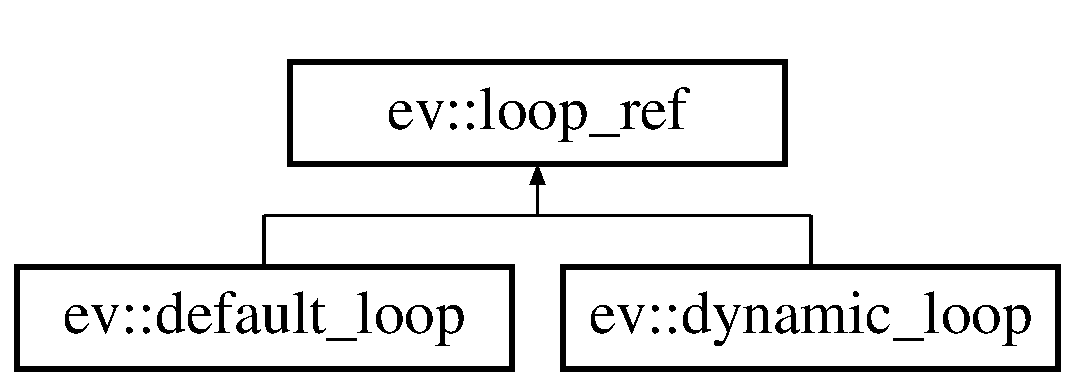
\includegraphics[height=2.000000cm]{structev_1_1loop__ref}
\end{center}
\end{figure}
\subsection*{Public Member Functions}
\begin{DoxyCompactItemize}
\item 
\hypertarget{structev_1_1loop__ref_af8f35791dbfc13235d5da3261e0f221b}{}\label{structev_1_1loop__ref_af8f35791dbfc13235d5da3261e0f221b} 
{\bfseries loop\+\_\+ref} (E\+V\+\_\+P)  throw ()
\item 
\hypertarget{structev_1_1loop__ref_aead905548b6ac07d97654fa7d4a569c4}{}\label{structev_1_1loop__ref_aead905548b6ac07d97654fa7d4a569c4} 
bool {\bfseries operator==} (const \hyperlink{structev_1_1loop__ref}{loop\+\_\+ref} \&other) const  throw ()
\item 
\hypertarget{structev_1_1loop__ref_a441765d1f27280dcba684fab2654e15b}{}\label{structev_1_1loop__ref_a441765d1f27280dcba684fab2654e15b} 
bool {\bfseries operator!=} (const \hyperlink{structev_1_1loop__ref}{loop\+\_\+ref} \&other) const  throw ()
\item 
\hypertarget{structev_1_1loop__ref_a9957eca84f0bf44875cbcabf72ecd81e}{}\label{structev_1_1loop__ref_a9957eca84f0bf44875cbcabf72ecd81e} 
bool {\bfseries operator==} (const E\+V\+\_\+P) const  throw ()
\item 
\hypertarget{structev_1_1loop__ref_abd695290d3cd6324eba73824d213b05e}{}\label{structev_1_1loop__ref_abd695290d3cd6324eba73824d213b05e} 
bool {\bfseries operator!=} (const E\+V\+\_\+P) const  throw ()
\item 
\hypertarget{structev_1_1loop__ref_aaefad67b40311ad68544d604d484dcbb}{}\label{structev_1_1loop__ref_aaefad67b40311ad68544d604d484dcbb} 
{\bfseries operator struct ev\+\_\+loop $\ast$} () const  throw ()
\item 
\hypertarget{structev_1_1loop__ref_af0618b351074be5243c985fccb470896}{}\label{structev_1_1loop__ref_af0618b351074be5243c985fccb470896} 
{\bfseries operator const struct ev\+\_\+loop $\ast$} () const  throw ()
\item 
\hypertarget{structev_1_1loop__ref_ab803c7d23963803c24ae201abb862aed}{}\label{structev_1_1loop__ref_ab803c7d23963803c24ae201abb862aed} 
bool {\bfseries is\+\_\+default} () const  throw ()
\item 
\hypertarget{structev_1_1loop__ref_aac842842270f64dbbc2ce71b033e0be7}{}\label{structev_1_1loop__ref_aac842842270f64dbbc2ce71b033e0be7} 
void {\bfseries loop} (int flags=0)
\item 
\hypertarget{structev_1_1loop__ref_aec8590666ff6a3fe0a09c1ba86c5fd6a}{}\label{structev_1_1loop__ref_aec8590666ff6a3fe0a09c1ba86c5fd6a} 
void {\bfseries unloop} (how\+\_\+t how=O\+NE)  throw ()
\item 
\hypertarget{structev_1_1loop__ref_a895c5422c6012224bd99ab30ae13caa6}{}\label{structev_1_1loop__ref_a895c5422c6012224bd99ab30ae13caa6} 
void {\bfseries run} (int flags=0)
\item 
\hypertarget{structev_1_1loop__ref_a579d5108904f34c7faac0b41336dfcf3}{}\label{structev_1_1loop__ref_a579d5108904f34c7faac0b41336dfcf3} 
void {\bfseries break\+\_\+loop} (how\+\_\+t how=O\+NE)  throw ()
\item 
\hypertarget{structev_1_1loop__ref_aa46f607fc2bf3ac6834b8b2df9596398}{}\label{structev_1_1loop__ref_aa46f607fc2bf3ac6834b8b2df9596398} 
void {\bfseries post\+\_\+fork} ()  throw ()
\item 
\hypertarget{structev_1_1loop__ref_a1e18db43676887445aeb97748c7f4082}{}\label{structev_1_1loop__ref_a1e18db43676887445aeb97748c7f4082} 
unsigned int {\bfseries backend} () const  throw ()
\item 
\hypertarget{structev_1_1loop__ref_afecb6dbce9db53575e7a3a8fb8fcf9a6}{}\label{structev_1_1loop__ref_afecb6dbce9db53575e7a3a8fb8fcf9a6} 
tstamp {\bfseries now} () const  throw ()
\item 
\hypertarget{structev_1_1loop__ref_a09bebb58fbbcf040b519d664add29722}{}\label{structev_1_1loop__ref_a09bebb58fbbcf040b519d664add29722} 
void {\bfseries ref} ()  throw ()
\item 
\hypertarget{structev_1_1loop__ref_ab1dddfeae1c8fcdded9dd08afff3940d}{}\label{structev_1_1loop__ref_ab1dddfeae1c8fcdded9dd08afff3940d} 
void {\bfseries unref} ()  throw ()
\item 
\hypertarget{structev_1_1loop__ref_a8aba353209992f883e7fe83c718a557c}{}\label{structev_1_1loop__ref_a8aba353209992f883e7fe83c718a557c} 
unsigned int {\bfseries iteration} () const  throw ()
\item 
\hypertarget{structev_1_1loop__ref_aa53dd1b61f1ee44058a10a590ce4f982}{}\label{structev_1_1loop__ref_aa53dd1b61f1ee44058a10a590ce4f982} 
unsigned int {\bfseries depth} () const  throw ()
\item 
\hypertarget{structev_1_1loop__ref_a6b085b1d677aaedc5bfab9e19682191a}{}\label{structev_1_1loop__ref_a6b085b1d677aaedc5bfab9e19682191a} 
void {\bfseries set\+\_\+io\+\_\+collect\+\_\+interval} (tstamp interval)  throw ()
\item 
\hypertarget{structev_1_1loop__ref_a29069e561a298346dbcabc0a6a35ed66}{}\label{structev_1_1loop__ref_a29069e561a298346dbcabc0a6a35ed66} 
void {\bfseries set\+\_\+timeout\+\_\+collect\+\_\+interval} (tstamp interval)  throw ()
\item 
\hypertarget{structev_1_1loop__ref_a15e082bc546385d1c465c46ec2f5e57c}{}\label{structev_1_1loop__ref_a15e082bc546385d1c465c46ec2f5e57c} 
void {\bfseries once} (int fd, int events, tstamp timeout, void($\ast$cb)(int, void $\ast$), void $\ast$arg=0)  throw ()
\item 
\hypertarget{structev_1_1loop__ref_a00791486a12936d4bc98cf060b2a87ae}{}\label{structev_1_1loop__ref_a00791486a12936d4bc98cf060b2a87ae} 
{\footnotesize template$<$class K , void(\+K\+::$\ast$)(int) method$>$ }\\void {\bfseries once} (int fd, int events, tstamp timeout, K $\ast$object)  throw ()
\item 
\hypertarget{structev_1_1loop__ref_a05d8ecf4b8df5de8ef2742eec6eee7b4}{}\label{structev_1_1loop__ref_a05d8ecf4b8df5de8ef2742eec6eee7b4} 
{\footnotesize template$<$class K $>$ }\\void {\bfseries once} (int fd, int events, tstamp timeout, K $\ast$object)  throw ()
\item 
\hypertarget{structev_1_1loop__ref_a00791486a12936d4bc98cf060b2a87ae}{}\label{structev_1_1loop__ref_a00791486a12936d4bc98cf060b2a87ae} 
{\footnotesize template$<$class K , void(\+K\+::$\ast$)() method$>$ }\\void {\bfseries once} (int fd, int events, tstamp timeout, K $\ast$object)  throw ()
\item 
\hypertarget{structev_1_1loop__ref_ad00f4c273e5c2531392ef3909992b888}{}\label{structev_1_1loop__ref_ad00f4c273e5c2531392ef3909992b888} 
{\footnotesize template$<$void($\ast$)(int) cb$>$ }\\void {\bfseries once} (int fd, int events, tstamp timeout)  throw ()
\item 
\hypertarget{structev_1_1loop__ref_ad00f4c273e5c2531392ef3909992b888}{}\label{structev_1_1loop__ref_ad00f4c273e5c2531392ef3909992b888} 
{\footnotesize template$<$void($\ast$)() cb$>$ }\\void {\bfseries once} (int fd, int events, tstamp timeout)  throw ()
\item 
\hypertarget{structev_1_1loop__ref_ab9ee42bfaba2b1e86f797bc6dfbfd0dc}{}\label{structev_1_1loop__ref_ab9ee42bfaba2b1e86f797bc6dfbfd0dc} 
void {\bfseries feed\+\_\+fd\+\_\+event} (int fd, int revents)  throw ()
\item 
\hypertarget{structev_1_1loop__ref_ad398231ff9498cfa17bad40baf3ce928}{}\label{structev_1_1loop__ref_ad398231ff9498cfa17bad40baf3ce928} 
void {\bfseries feed\+\_\+signal\+\_\+event} (int signum)  throw ()
\end{DoxyCompactItemize}
\subsection*{Static Public Member Functions}
\begin{DoxyCompactItemize}
\item 
\hypertarget{structev_1_1loop__ref_a9e8f3b059640ed2a1c3eef5bd083c999}{}\label{structev_1_1loop__ref_a9e8f3b059640ed2a1c3eef5bd083c999} 
{\footnotesize template$<$class K , void(\+K\+::$\ast$)(int) method$>$ }\\static void {\bfseries method\+\_\+thunk} (int revents, void $\ast$arg)
\item 
\hypertarget{structev_1_1loop__ref_aa0129e98abbdea7d42f18809f1a1a539}{}\label{structev_1_1loop__ref_aa0129e98abbdea7d42f18809f1a1a539} 
{\footnotesize template$<$class K , void(\+K\+::$\ast$)() method$>$ }\\static void {\bfseries method\+\_\+noargs\+\_\+thunk} (int revents, void $\ast$arg)
\item 
\hypertarget{structev_1_1loop__ref_a78f26c622a851958fb753f0387f9c114}{}\label{structev_1_1loop__ref_a78f26c622a851958fb753f0387f9c114} 
{\footnotesize template$<$void($\ast$)(int) cb$>$ }\\static void {\bfseries simpler\+\_\+func\+\_\+thunk} (int revents, void $\ast$arg)
\item 
\hypertarget{structev_1_1loop__ref_a9114fcf7ef168f264abaf05dc7d76c44}{}\label{structev_1_1loop__ref_a9114fcf7ef168f264abaf05dc7d76c44} 
{\footnotesize template$<$void($\ast$)() cb$>$ }\\static void {\bfseries simplest\+\_\+func\+\_\+thunk} (int revents, void $\ast$arg)
\end{DoxyCompactItemize}
\subsection*{Public Attributes}
\begin{DoxyCompactItemize}
\item 
\hypertarget{structev_1_1loop__ref_abbf426c43deec8dad767439421985970}{}\label{structev_1_1loop__ref_abbf426c43deec8dad767439421985970} 
struct \hyperlink{structev__loop}{ev\+\_\+loop} $\ast$ {\bfseries E\+V\+\_\+\+AX}
\end{DoxyCompactItemize}


The documentation for this struct was generated from the following file\+:\begin{DoxyCompactItemize}
\item 
ev++.\+h\end{DoxyCompactItemize}

%--- End generated contents ---

% Index
\backmatter
\newpage
\phantomsection
\clearemptydoublepage
\addcontentsline{toc}{chapter}{Index}
\printindex

\end{document}
